\newpage
\setcounter{secnumdepth}{1}
\section{Mathematical model}

\begin{figure}[ht]
\centering
\subfigure{
	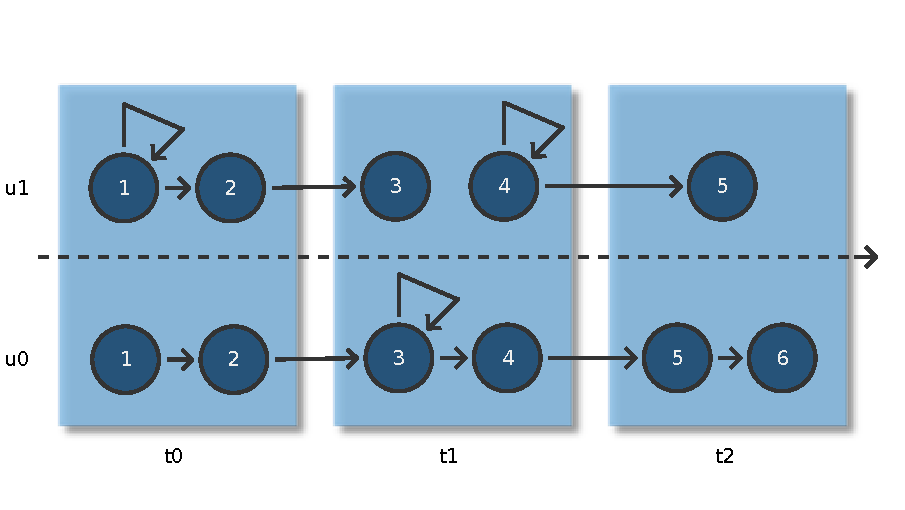
\includegraphics[scale =0.45] {mathematical_definition/images/dynamic_users.pdf}
	\label{fig:subfig11}
}
\caption[Optional caption for list of figures]{Dynamic and static user patterns}
\label{fig:fig1}
\end{figure}


The above figure shows two users ${u_0,u_1}$ repesented on the vertical axe, grouped by three time windows $t_o,t_1,t_2$. A time window is defined as $t_n$ where $n \in \{0,..,24\}$. Each $t_n$ groups the comunnications traces of the whole set of users in a 60 minutes range. 
\\More formally, an user trace is defined as follows:
$$ \vec{T}_u_t = (p_0,p_1,...,p_n)  $$ where, 
$p_n \in \mathbb{R}^2$ , 
$n \geq 2 $, 
$t$ is a temporal window range and ,
$u$ the unique user id.
\\
For instance, $ \vec{T}_0_0 = (p_1,p_2)  $, $ \vec{T}_1_0 = (p_1,p_1,p_2)  $ and so on.
\\
\\
Also, two functions are defined in order to measure the distance \citep{distance}, given a set of points in spherical coordinates (i.e.: $\text{user}_u_t$):
$$D(p_0, p_1) = \text{acos}( \sin(\phi(p_0^0)) * \sin(\phi(p_1^0)) * \cos(\theta(p_0^1) - \theta(p_1^1)) + \cos(\phi(p_0^0)) * \cos(\phi(p_1^0)))  $$
where:
$$ \phi(x) = (90 - x) * \frac{\pi}{180}$$
$$ \theta(x) = x  * \frac{\pi}{180}$$
therefore the function related with distance as defined as follow [result in Km]:
$$U(u,t) = \dysplaystyle 6373 * \sum_{i=0}^{n-1} D(\vec{T}_u_t^i, \vec{T}_u_t^{i+1}) $$
\\
The second function is related with the number of antenna connections into a trace, the key point is to count only the dinamic transitions, i.e.: remove the self edges over a given trace as follows:
\\
\begin{equation*}
\text{S}(p_0, p_1) = \left \{
\begin{matrix}
0 & \text{if } D(p_0, p_1) = 0 \\
1 & \text{if } D(p_0, p_1) > 0 \\
\end{matrix} \right.
\end{equation*}
therefore, the function is defined as follows:
$$N(u,t) = \dysplaystyle \sum_{i=0}^{n-1} S(\vec{T}_u_t^i, \vec{T}_u_t^{i+1})$$
